\chapter{Projeto}
\label{cap:proj}

Neste trabalho será proposta a implementação de estratégias de otimização de classificação de imagens hiperespectrais utilizando CNNs 1D combinadas com técnicas de segmentação espacial. A partir de arquiteturas e algoritmos encontrados na literatura, procura-se fazer uma análise com base nas métricas elencadas neste projeto. O capítulo está organizado da seguinte forma: inicialmente é apresentada a visão geral do sistema proposto. Na sequência, são dispostas as premissas que norteiam o desenvolvimento. Posteriormente, são descritos os materiais e métodos utilizados, incluindo o detalhamento da arquitetura do sistema e dos algoritmos implementados. Ao fim, são apresentados os requisitos levantados, o plano de verificação, a análise de riscos e o cronograma de atividades.

\section{Visão Geral}

Serão implementadas estratégias de otimização de classificação de imagens hiperespectrais utilizando CNNs 1D combinadas com técnicas de segmentação espacial. O projeto visa paralelizar o processamento e automatizar o ajuste de hiperparâmetros tanto do modelo de classificação quanto dos algoritmos de segmentação. As técnicas específicas implementadas são detalhadas na \autoref{subsec:algoritmos}.

Para a avaliação da eficácia e do custo computacional das otimizações propostas, serão utilizados três datasets de referência na área: Indian Pines, Salinas Valley e University of Pavia. Os detalhes da campanha de experimentos são abordados na \autoref{subsec:campanhaExperimental}.

A \autoref{fig:visaoGeral} sumariza a relação entre os principais componentes do sistema proposto. A arquitetura híbrida processa simultaneamente as características espectrais via CNN 1D e as características espaciais via algoritmos de segmentação, realizando a fusão dos dados através de uma camada de concatenação. O processo de otimização de hiperparâmetros é controlado por algoritmos automatizados que ajustam tanto os parâmetros da rede neural quanto os parâmetros de segmentação.

\begin{figure}[H]
    \centering
    \captionsetup{justification=centering}
    \caption{Principais componentes do projeto}
     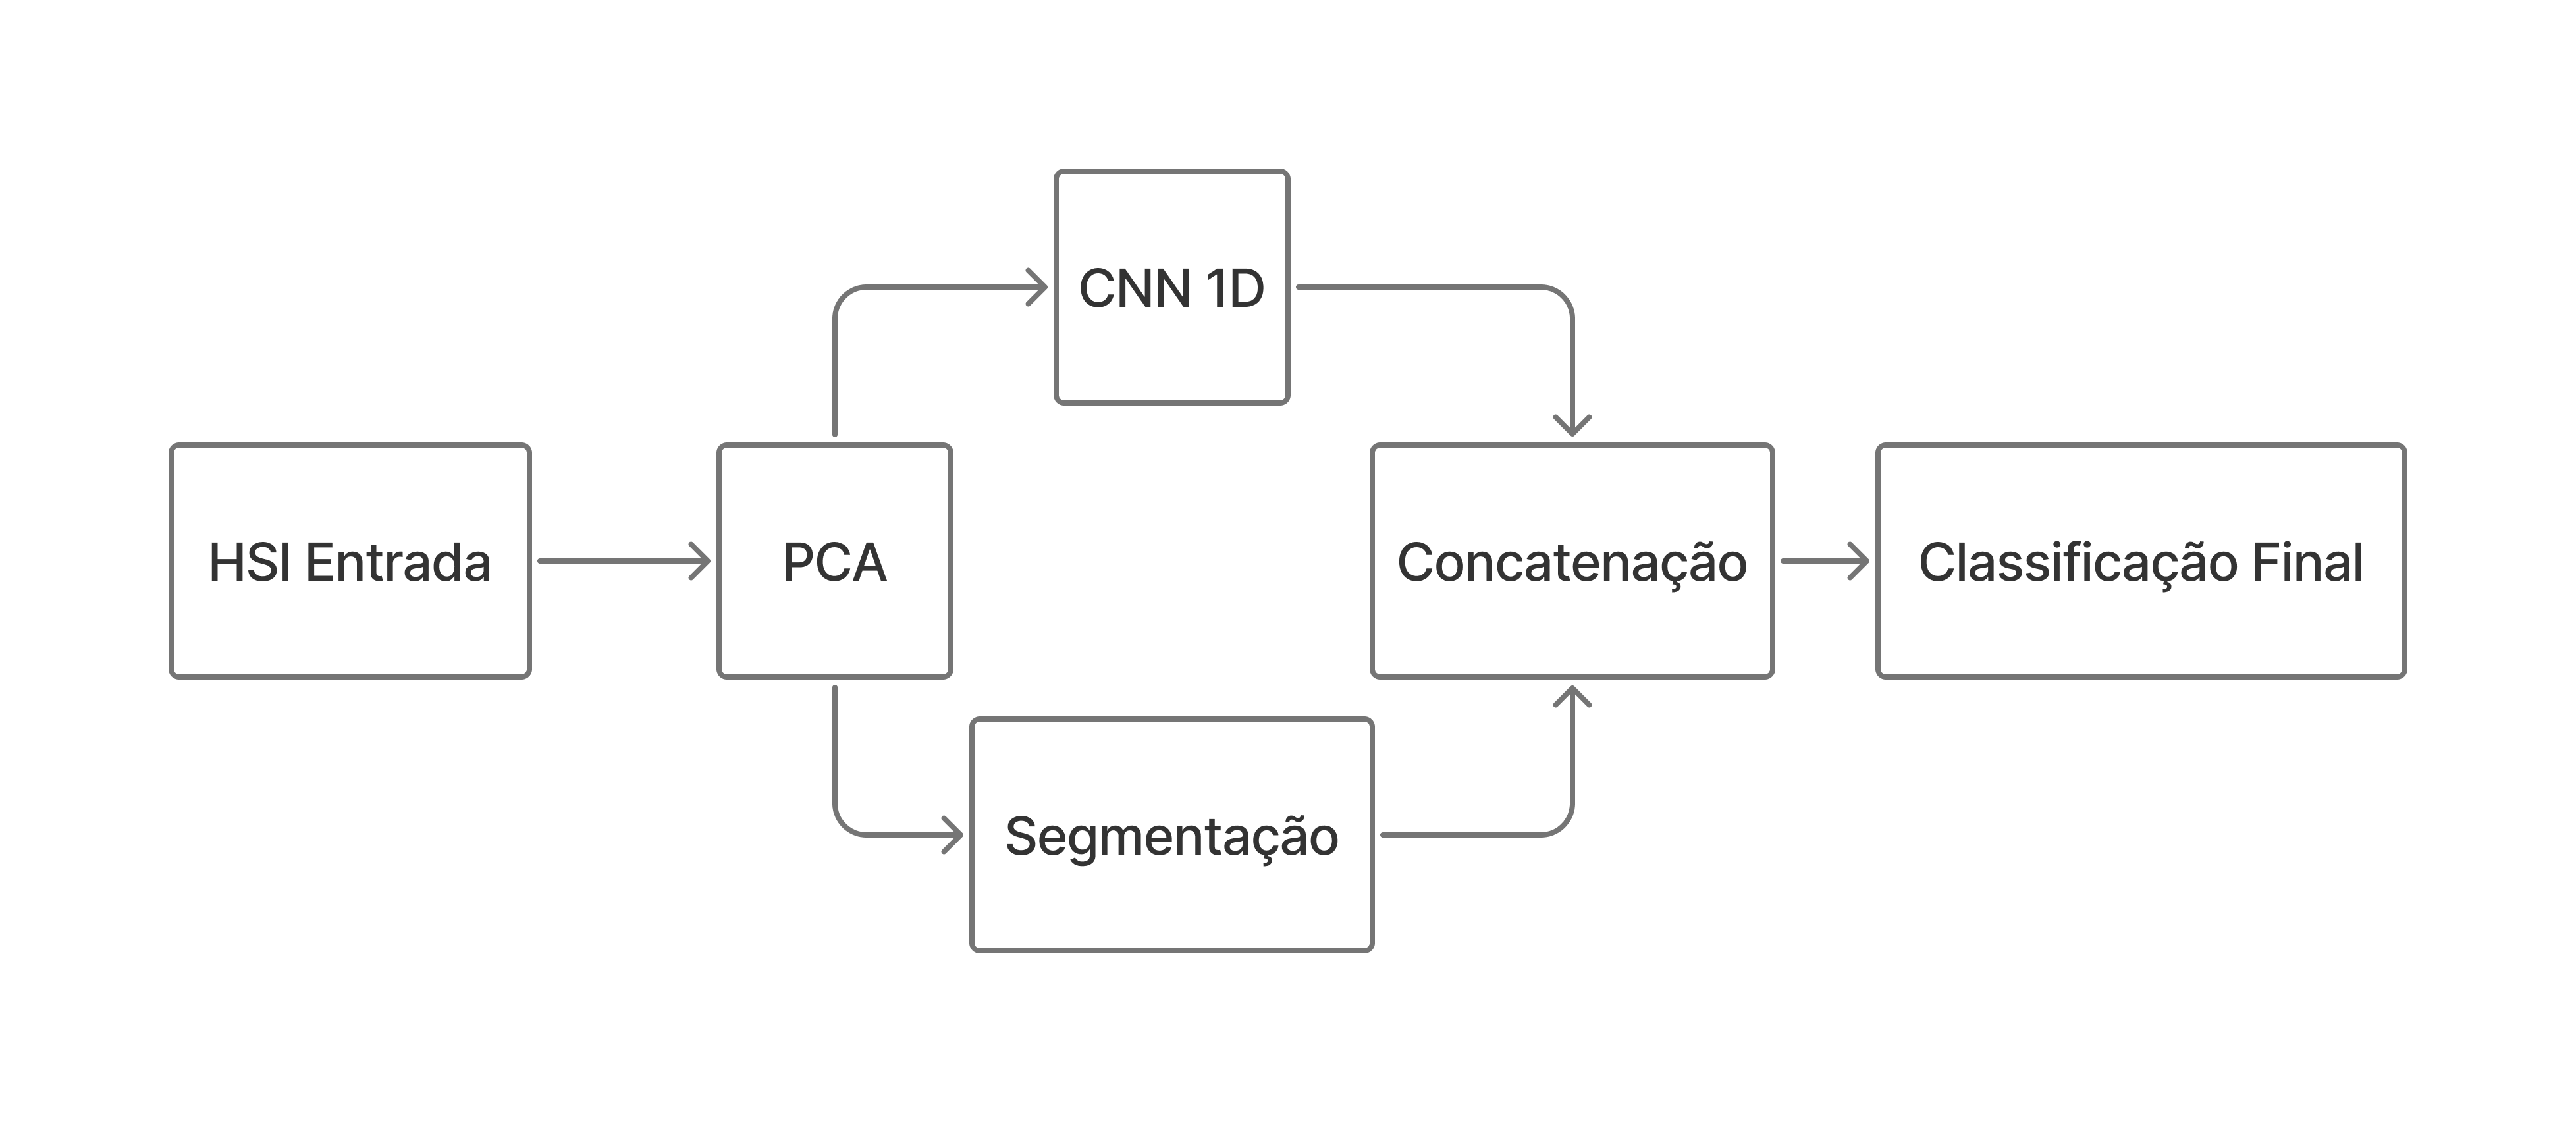
\includegraphics[width=0.8\textwidth]{assets/projeto/visaoGeral.png}\\
    \captionsetup{justification=raggedright}
    \caption*{Fonte: Elaborada pelo autor}
    \label{fig:visaoGeral}
\end{figure}

\section{Premissas}

O trabalho parte do pressuposto de que a arquitetura base proposta por \cite{Souza2023}, que combina CNN 1D com segmentação SEEDS, apresenta gargalos de processamento identificados que podem ser mitigados através de técnicas de paralelização e otimização automática de hiperparâmetros. Especificamente, assume-se que o processamento sequencial, particularmente na etapa de restrição espectral que consome mais de dois terços do tempo de execução, pode ser significativamente acelerado.

Será considerado que os três datasets selecionados (Indian Pines com 21k pixels e 16 classes, Salinas Valley com 111k pixels e 16 classes, e University of Pavia com 207k pixels e 9 classes) são representativos o suficiente para validar as melhorias propostas e permitir comparações diretas com trabalhos relacionados da literatura.

Presume-se que a separação de 85\% das amostras para treinamento e 15\% para validação e teste, conforme adotado na literatura, é adequada para avaliar o desempenho dos modelos.

Quanto à otimização de hiperparâmetros, será assumido que técnicas de busca automatizada como Grid Search e Otimização Bayesiana são capazes de encontrar configurações próximas ao ótimo global dentro de um espaço de busca adequadamente definido.

Em relação ao processamento paralelo, presume-se que a paralelização das etapas de segmentação e classificação espectral pode reduzir significativamente o tempo total de processamento, dado que essas operações apresentam independência de dados durante parte do fluxo de execução.

Portanto, os resultados extraídos dos experimentos controlados serão capazes de demonstrar os ganhos relativos introduzidos pelas otimizações propostas e poderão orientar aplicações em cenários reais de processamento de imagens hiperespectrais.

\section{Metodologia}

\subsection{Materiais}

\subsubsection{Ambiente Computacional e Ferramentas}

O desenvolvimento e experimentação serão realizados utilizando a linguagem Python com as seguintes bibliotecas principais: TensorFlow/Keras ou PyTorch para implementação da CNN 1D, Scikit-Learn para pré-processamento (PCA) e métricas, OpenCV para manipulação de imagens, e Ray Tune para otimização de hiperparâmetros.

Os experimentos computacionalmente intensivos serão executados em ambiente de computação de alto desempenho (HPC) ou Google Colab Pro com acesso a GPUs. Para experimentos preliminares e desenvolvimento, será utilizado ambiente local com CPU multi-core.

\subsubsection{Datasets Hiperespectrais}

Serão utilizados três datasets públicos de imagens hiperespectrais amplamente referenciados na literatura, conforme ilustrados nas Figuras \ref{fig:indian_pines}, \ref{fig:salinas_valley} e \ref{fig:pavia_university}.

O dataset \textbf{Indian Pines} (Figura \ref{fig:indian_pines}) representa uma área agrícola capturada em 1992 pelo sensor AVIRIS no noroeste de Indiana. A imagem possui dimensões de 145×145 pixels com resolução espacial de 20 metros por pixel e classifica 16 tipos diferentes de vegetação. Das 224 bandas originais capturadas pelo sensor, foram utilizadas 200 bandas espectrais na faixa de 400 a 2500 nanômetros com intervalos de 10 nanômetros, após a remoção de 4 bandas nulas e 20 bandas comprometidas pela absorção atmosférica de água. A visualização apresenta a composição em falsa-cor à esquerda, o mapa de classificação terrestre ao centro, e a legenda com as 16 classes que incluem diferentes tipos de culturas agrícolas (alfafa, milho, soja, trigo), pastagens e áreas construídas \cite{LabanReduced3D}.

\begin{figure}[H]
    \centering
    \captionsetup{justification=centering}
    \caption{Indian Pines: composição falsa-cor, mapa de verdade terrestre e legenda}
    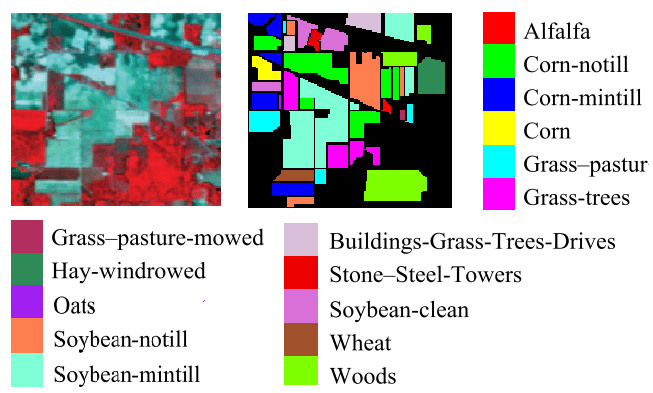
\includegraphics[width=0.8\textwidth]{assets/projeto/indian-pines_dataset_visualization.png}\\
    \captionsetup{justification=raggedright}
    \caption*{Fonte: \citefigure{LabanReduced3D}}
    \label{fig:indian_pines}
\end{figure}

O dataset \textbf{Salinas Valley} (Figura \ref{fig:salinas_valley}) foi capturado pelos sensores AVIRIS na região do Vale de Salinas, Califórnia, apresentando resolução espacial de 3,7 metros por pixel. A imagem possui dimensões de 512×217 pixels e originalmente continha 224 bandas espectrais. Após a remoção de 20 bandas afetadas pela absorção de água, restaram 204 bandas espectrais utilizáveis para análise. O dataset classifica todos os pixels em 16 categorias distintas, predominantemente relacionadas a diferentes tipos de culturas agrícolas e cobertura do solo, totalizando aproximadamente 111.104 pixels rotulados. A imagem (a) mostra a composição falsa-cor da área agrícola, (b) apresenta o mapa de classificação com as diferentes culturas, e (c) exibe a legenda contendo 16 classes que incluem diversos tipos de brócolis, alface romana em diferentes estágios, vinhedos e outras culturas \cite{Li2022Directionally}.

\begin{figure}[H]
    \centering
    \captionsetup{justification=centering}
    \caption{Salinas Valley: (a) falsa-cor, (b) verdade terrestre, (c) legenda}
    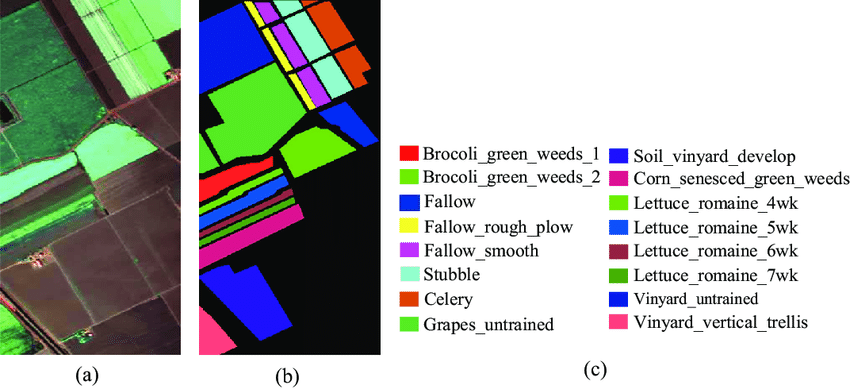
\includegraphics[width=0.85\textwidth]{assets/projeto/salinas_valley_dataset_visualization.png}\\
    \captionsetup{justification=raggedright}
    \caption*{Fonte: \citefigure{Li2022Directionally}}
    \label{fig:salinas_valley}
\end{figure}

Por fim, o dataset \textbf{University of Pavia} (Figura \ref{fig:pavia_university}) representa uma área urbana da Universidade de Pavia, Itália, capturada em 2003 pelo sensor ROSIS. A imagem possui dimensões de 610×340 pixels com resolução espacial de 1,3 metros por pixel, classificando todos os pixels em 9 categorias de cobertura urbana. Das 115 bandas espectrais originais capturadas na faixa de comprimento de onda entre 0,43 e 0,86 micrômetros (430 a 860 nanômetros), foram utilizadas 103 bandas após a remoção de 12 bandas contaminadas por ruído, totalizando aproximadamente 207.400 pixels rotulados. A visualização mostra em (a) a composição falsa-cor da área universitária, em (b) o mapa de classificação com delimitação precisa das estruturas urbanas, e a legenda contendo 9 classes que incluem asfalto, prados, cascalho, árvores, chapas metálicas pintadas, solo exposto, betume, tijolos autoblocantes e sombras \cite{Qi2019Spectral}.

\begin{figure}[H]
    \centering
    \captionsetup{justification=centering}
    \caption{University of Pavia: (a) falsa-cor, (b) verdade terrestre e legenda}
    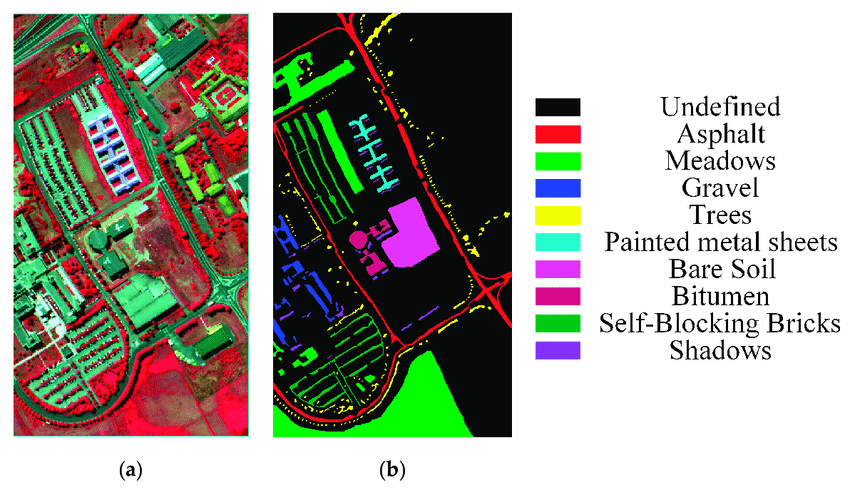
\includegraphics[width=0.7\textwidth]{assets/projeto/university_of_pavia_dataset_visualization.png}\\
    \captionsetup{justification=raggedright}
    \caption*{Fonte: \citefigure{Qi2019Spectral}}
    \label{fig:pavia_university}
\end{figure}

Para versionamento de código será utilizado Git, e para documentação e reprodutibilidade dos experimentos será mantido registro detalhado de todas as configurações utilizadas através de arquivos de configuração e notebooks Jupyter.

\subsection{Métodos}

Serão utilizadas as seguintes técnicas e estratégias de otimização: paralelização do processamento espacial e espectral, otimização automática de hiperparâmetros (Grid Search e Otimização Bayesiana), comparação de diferentes algoritmos de segmentação como SEEDS, LSC, Watershed, e técnicas de redução dimensional via PCA. O detalhamento específico de cada técnica é abordado em maior detalhe na \autoref{subsec:algoritmos}.

A coleta de métricas será realizada utilizando as ferramentas nativas do TensorFlow/Keras e Pytorch para monitoramento de treinamento, bibliotecas de profiling do Python para medição de tempo de execução, e utilitários do sistema para medição de uso de memória. As métricas principais incluem: Acurácia Global (OA), Acurácia Média (AA), coeficiente Kappa, tempo de treinamento, tempo de inferência, uso de memória, e speedup obtido com paralelização.

A fim de promover a reutilização de código e facilitar a reprodução dos experimentos, será implementado um framework modular que abstrai os componentes principais do sistema: módulo de pré-processamento, módulo de segmentação, módulo de classificação CNN, módulo de fusão, e módulo de avaliação. A interação entre esses módulos é abordada em maior detalhe na \autoref{subsec:arquitetura}.

\section{Análise de Requisitos}
\label{sec:req}

\begin{quadro}[H]
    \centering
    \caption{Requisitos funcionais}
    \begin{tabular}{|p{0.125\textwidth}|p{0.8\textwidth}|}
        \hline
        \rowcolor[HTML]{C0C0C0}
        \textbf{Requisito} & \textbf{Descrição}  \\
        \hline
        
        \textbf{RF01} & A arquitetura deve classificar HSIs utilizando CNN 1D para extração de características espectrais \\ 
        \hline

        \textbf{RF02} & A arquitetura deve implementar algoritmos de segmentação espacial \\
        \hline

        \textbf{RF03} & A arquitetura deve realizar fusão de dados espectrais e espaciais \\
        \hline
        
        \textbf{RF04} & O sistema deve implementar otimização automática de hiperparâmetros \\
        \hline

        \textbf{RF05} & O sistema deve produzir métricas de desempenho e custo computacional \\
        \hline
        
        \textbf{RF06} & O sistema deve implementar paralelização do processamento espacial e espectral \\
        \hline
    \end{tabular}
    \label{tab:rf}
\end{quadro}

\begin{quadro}[H]
    \centering
    \caption{Requisitos não funcionais}
    \begin{tabular}{|p{0.125\textwidth}|p{0.8\textwidth}|}
       \hline
        \rowcolor[HTML]{C0C0C0}
        \textbf{Requisito} & \textbf{Descrição}  \\
        \hline
        
        \textbf{RNF01} & O classificador espectral deve ser uma CNN 1D baseada no modelo de \cite{Souza2023} e \cite{Viel10064297} \\
        \hline
        
        \textbf{RNF02} & Toda a arquitetura deve ser desenvolvida na linguagem de programação Python \\
        \hline

        \textbf{RNF03} & Para treinar, testar e validar o modelo deve ser utilizada a plataforma Google Colab ou ambiente HPC com GPU \\
        \hline

        \textbf{RNF04} & A fusão de dados deve ser realizada por concatenação dos segmentos espaciais com features espectrais na CNN \\
        \hline

        \textbf{RNF05} & A otimização automática de hiperparâmetros deve melhorar as métricas de acurácia (OA, AA, Kappa) em comparação ao ajuste manual \\
        \hline

        \textbf{RNF06} & O sistema deve produzir resultados reprodutíveis através de registro detalhado de configurações \\
        \hline
        
        \textbf{RNF07} & A paralelização deve alcançar redução mensurável no tempo de processamento em relação à implementação sequencial \\
        \hline
    \end{tabular}
    \label{tab:rnf}
\end{quadro}

\subsection{Arquitetura do Sistema} 
\label{subsec:arquitetura}

A arquitetura proposta segue um design modular que permite experimentação com diferentes configurações. A \autoref{fig:arquiteturaSistema} apresenta o diagrama de blocos detalhado do sistema completo.

\begin{figure}[H]
    \centering
    \captionsetup{justification=centering}
    \caption{Arquitetura modular do sistema}
     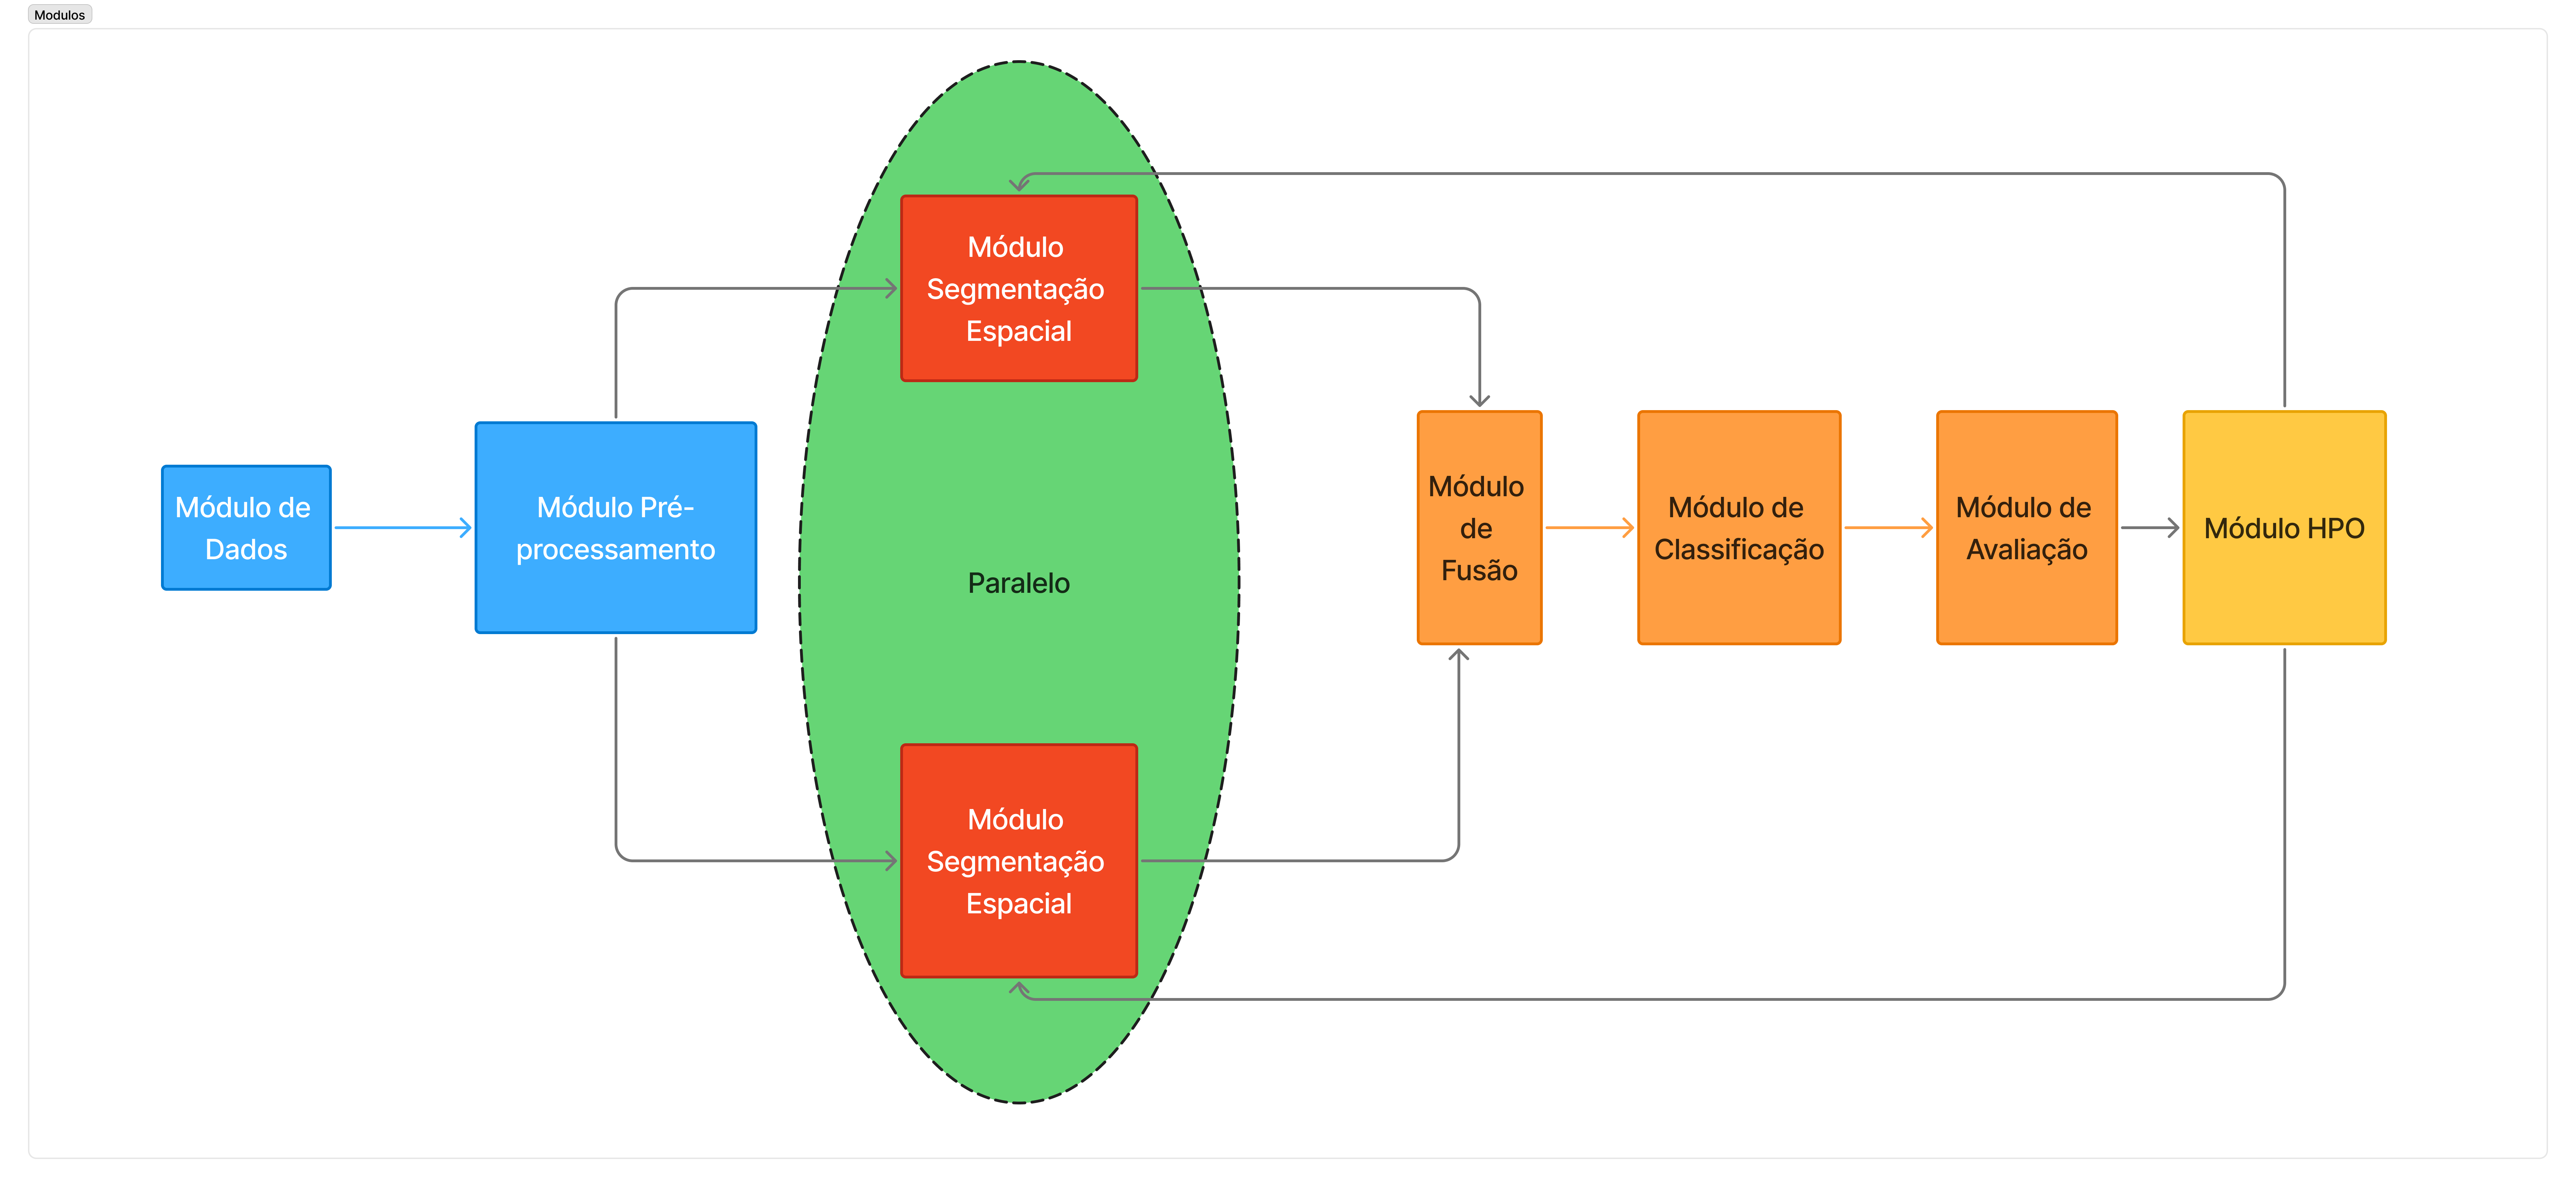
\includegraphics[width=0.9\textwidth]{assets/projeto/arquiteturaSistema.png}\\
    \captionsetup{justification=raggedright}
    \caption*{Fonte: Elaborada pelo autor}
    \label{fig:arquiteturaSistema}
\end{figure}

A arquitetura proposta organiza-se em módulos funcionais que operam de forma integrada. O Módulo de Dados é responsável pelo carregamento e preparação dos datasets, abstraindo as diferenças entre formatos distintos e fornecendo uma interface unificada para o sistema, além de realizar a separação dos conjuntos de treino, validação e teste com base em \citefigure{Souza2023},\citefigure{Viel10064297}.

O processamento dos dados ocorre em duas frentes paralelas. De um lado, o Módulo de Pré-processamento aplica a técnica de PCA para redução dimensional, transformando o hipercubo espectral original em um conjunto reduzido de componentes principais cujo número pode ser configurado conforme necessário. Do outro, o Módulo de Segmentação Espacial implementa os algoritmos SEEDS, LSC e Watershed de forma intercambiável, produzindo mapas de superpixels que capturam a estrutura espacial das imagens.

As características espectrais resultantes do pré-processamento são então alimentadas ao Módulo CNN 1D, que implementa uma rede neural convolucional unidimensional com arquitetura configurável, composta por camadas de convolução 1D seguidas de camadas densas totalmente conectadas. Este módulo extrai características discriminativas de cada pixel a partir de sua assinatura espectral.

O Módulo de Fusão realiza a concatenação entre as características espectrais extraídas pela CNN 1D e os rótulos de superpixels provenientes da segmentação espacial, unindo as informações complementares em um único vetor de características. Essas características fusionadas são então processadas pelo Módulo de Classificação, que realiza a predição final das classes para cada pixel da imagem.

O Módulo de Avaliação quantifica o desempenho do sistema através de métricas de acurácia e custo computacional. Por fim, o Módulo de Otimização de Hiperparâmetros coordena a busca automática dos melhores parâmetros tanto para os algoritmos de segmentação quanto para a arquitetura da CNN, utilizando técnicas como Grid Search ou Otimização Bayesiana para maximizar o desempenho global do sistema.

\subsection{Algoritmos e Técnicas} 
\label{subsec:algoritmos}

Para a implementação da funcionalidade de otimização e classificação de imagens hiperespectrais, técnicas de deep learning, processamento de imagens e otimização automática serão combinadas. O detalhamento sobre a implementação será abordado nesta seção.

\subsubsection{Redução Dimensional via PCA}

A técnica de Análise de Componentes Principais (PCA) será aplicada para reduzir a dimensionalidade espectral das imagens hiperespectrais. Dado um conjunto de dados com $n$ bandas espectrais, o PCA identifica as $k$ componentes principais (onde $k < n$) que capturam a maior variância dos dados.

\subsubsection{Rede Neural Convolucional 1D (CNN 1D)}

A arquitetura da CNN 1D é projetada para processar as características espectrais unidimensionais de cada pixel. A arquitetura base consiste em:

\begin{itemize}
    \item 4 camadas convolucionais 1D com 16, 32, 64 e 128 filtros respectivamente
    \item Função de ativação ReLU após cada camada convolucional
    \item Operações de max-pooling para redução dimensional
    \item 3 camadas densas (totalmente conectadas) com dropout para regularização
    \item Camada de saída com ativação softmax para classificação multi-classe
\end{itemize}

\begin{figure}[H]
    \centering
    \captionsetup{justification=centering}
    \caption{Arquitetura detalhada da CNN 1D}
    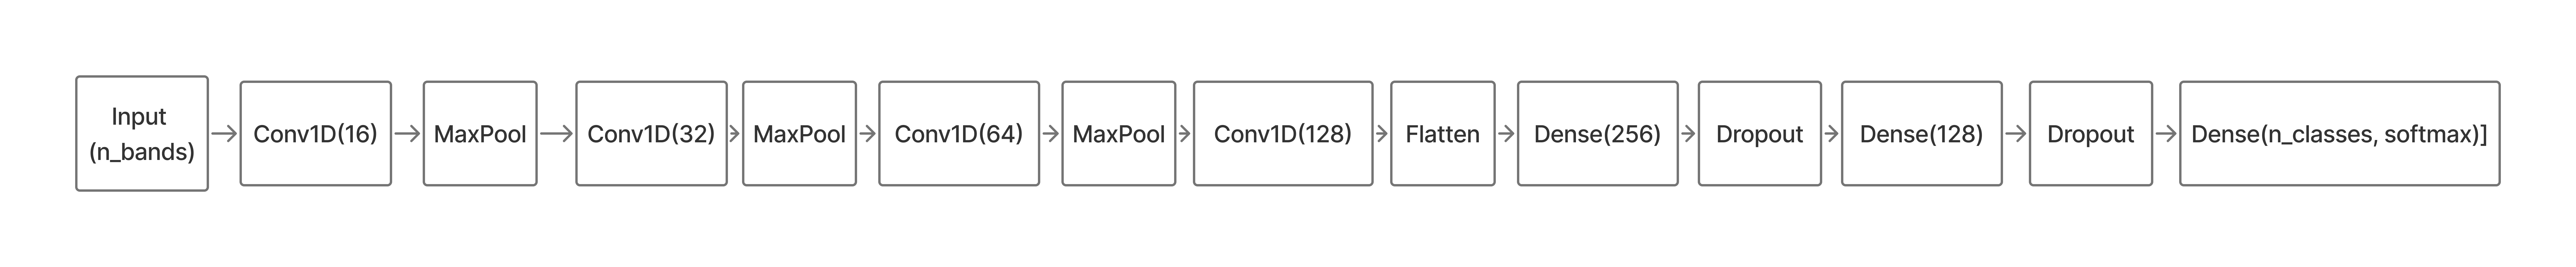
\includegraphics[width=0.9\textwidth]{assets/projeto/arquiteturaCNN.png}\\
    \captionsetup{justification=raggedright}
    \caption*{Fonte: Elaborada pelo autor}
    \label{fig:arquiteturaCNN}
\end{figure}

Os hiperparâmetros da rede (número de filtros, tamanho dos kernels, taxa de dropout, taxa de aprendizado, otimizador) serão otimizados automaticamente através do módulo de HPO.

\subsubsection{Algoritmos de Segmentação Espacial}

Três algoritmos de segmentação serão implementados e comparados:

\textbf{SEEDS (Superpixels Extracted via Energy-Driven Sampling)}: Algoritmo baseado em crescimento de regiões que busca minimizar uma função de energia. Os principais parâmetros ajustáveis são: número desejado de superpixels, número de iterações, e número de níveis de refinamento \cite{bergh2013seedssuperpixelsextractedenergydriven}.

\textbf{LSC (Linear Spectral Clustering)}: Algoritmo que realiza clustering espectral considerando tanto informação de cor quanto de posição espacial. Parâmetros principais: número de superpixels, peso da regularização espacial, e número de iterações \cite{Zhengqin7298741}.

\textbf{Watershed}: Algoritmo clássico de segmentação baseado em morfologia matemática que trata a imagem como uma superfície topográfica. Parâmetros: método de marcação de sementes e nível de compactação \cite{Najman546254}.

Cada algoritmo será executado sobre as três primeiras componentes principais obtidas via PCA, gerando um mapa de superpixels que identifica regiões espacialmente coerentes na imagem.

\subsubsection{Fusão de Características por Concatenação}

A fusão das características espectrais (extraídas pela CNN 1D) com as características espaciais (rótulos de superpixels) é realizada através de uma camada de concatenação \cite{Souza2023}. Para cada pixel:

\begin{enumerate}
    \item A CNN 1D extrai um vetor de características espectrais $\mathbf{f}_{spectral} \in \mathbb{R}^{d}$
    \item O algoritmo de segmentação atribui um rótulo de superpixel $l_{spatial} \in \{1, 2, ..., N_{superpixels}\}$
    \item O rótulo espacial é codificado como vetor one-hot $\mathbf{f}_{spatial} \in \mathbb{R}^{N_{superpixels}}$
    \item As características são concatenadas: $\mathbf{f}_{fused} = [\mathbf{f}_{spectral}, \mathbf{f}_{spatial}]$
\end{enumerate}

\begin{figure}[H]
    \centering
    \captionsetup{justification=centering}
    \caption{Processo de fusão por concatenação}
    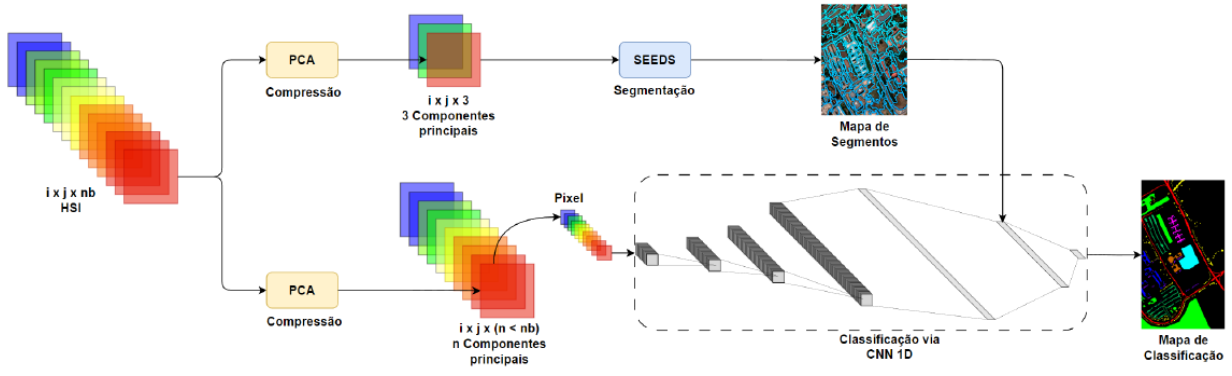
\includegraphics[width=0.9\textwidth]{assets/projeto/fusaoConcatenacao.png}\\
    \captionsetup{justification=raggedright}
    \caption*{Fonte: \citefigure{Souza2023}}
    \label{fig:fusaoConcatenacao}
\end{figure}

O vetor de características fusionadas é então alimentado a camadas densas adicionais que realizam a classificação final.

\subsubsection{Paralelização do Processamento}

Para acelerar o fluxo de processamento, a seguinte estratégia de paralelização será implementada, explorando a independência de dados entre as etapas de segmentação e classificação:

\textbf{Paralelização Inter-Etapas}: A segmentação espacial e a extração de características espectrais pela CNN são processos independentes que podem ser executados simultaneamente. Esta independência existe porque:
\begin{itemize}
    \item A segmentação opera sobre as componentes principais do PCA para gerar o mapa de superpixels, sem necessitar das features da CNN.
    \item A CNN 1D processa os vetores espectrais de cada pixel de forma independente da segmentação.
    \item Não há dependência de dados entre as duas operações até o momento da fusão.
\end{itemize}

Utilizando a biblioteca \texttt{multiprocessing} do Python para a segmentação (operação CPU-bound) e execução em GPU para a CNN (via CUDA cores), estas etapas são executadas em paralelo. A sincronização ocorre apenas no ponto de fusão, onde os resultados de ambas as operações são necessários.

\textbf{Paralelização Intra-Etapas}: Dentro da CNN 1D, o processamento em lotes (batches) permite aproveitar o paralelismo da GPU. As operações de convolução são intrinsecamente paralelizáveis porque cada elemento do mapa de características de saída pode ser calculado de forma independente dos demais, sem dependência de dados dentro da mesma camada. Esta propriedade permite que milhares de CUDA cores da GPU processem simultaneamente diferentes elementos de saída. Para a segmentação, alguns algoritmos podem processar diferentes regiões da imagem em paralelo utilizando múltiplas threads.

\begin{figure}[H]
    \centering
    \captionsetup{justification=centering}
    \caption{Estratégia de paralelização: fluxo sequencial versus fluxo paralelo}
    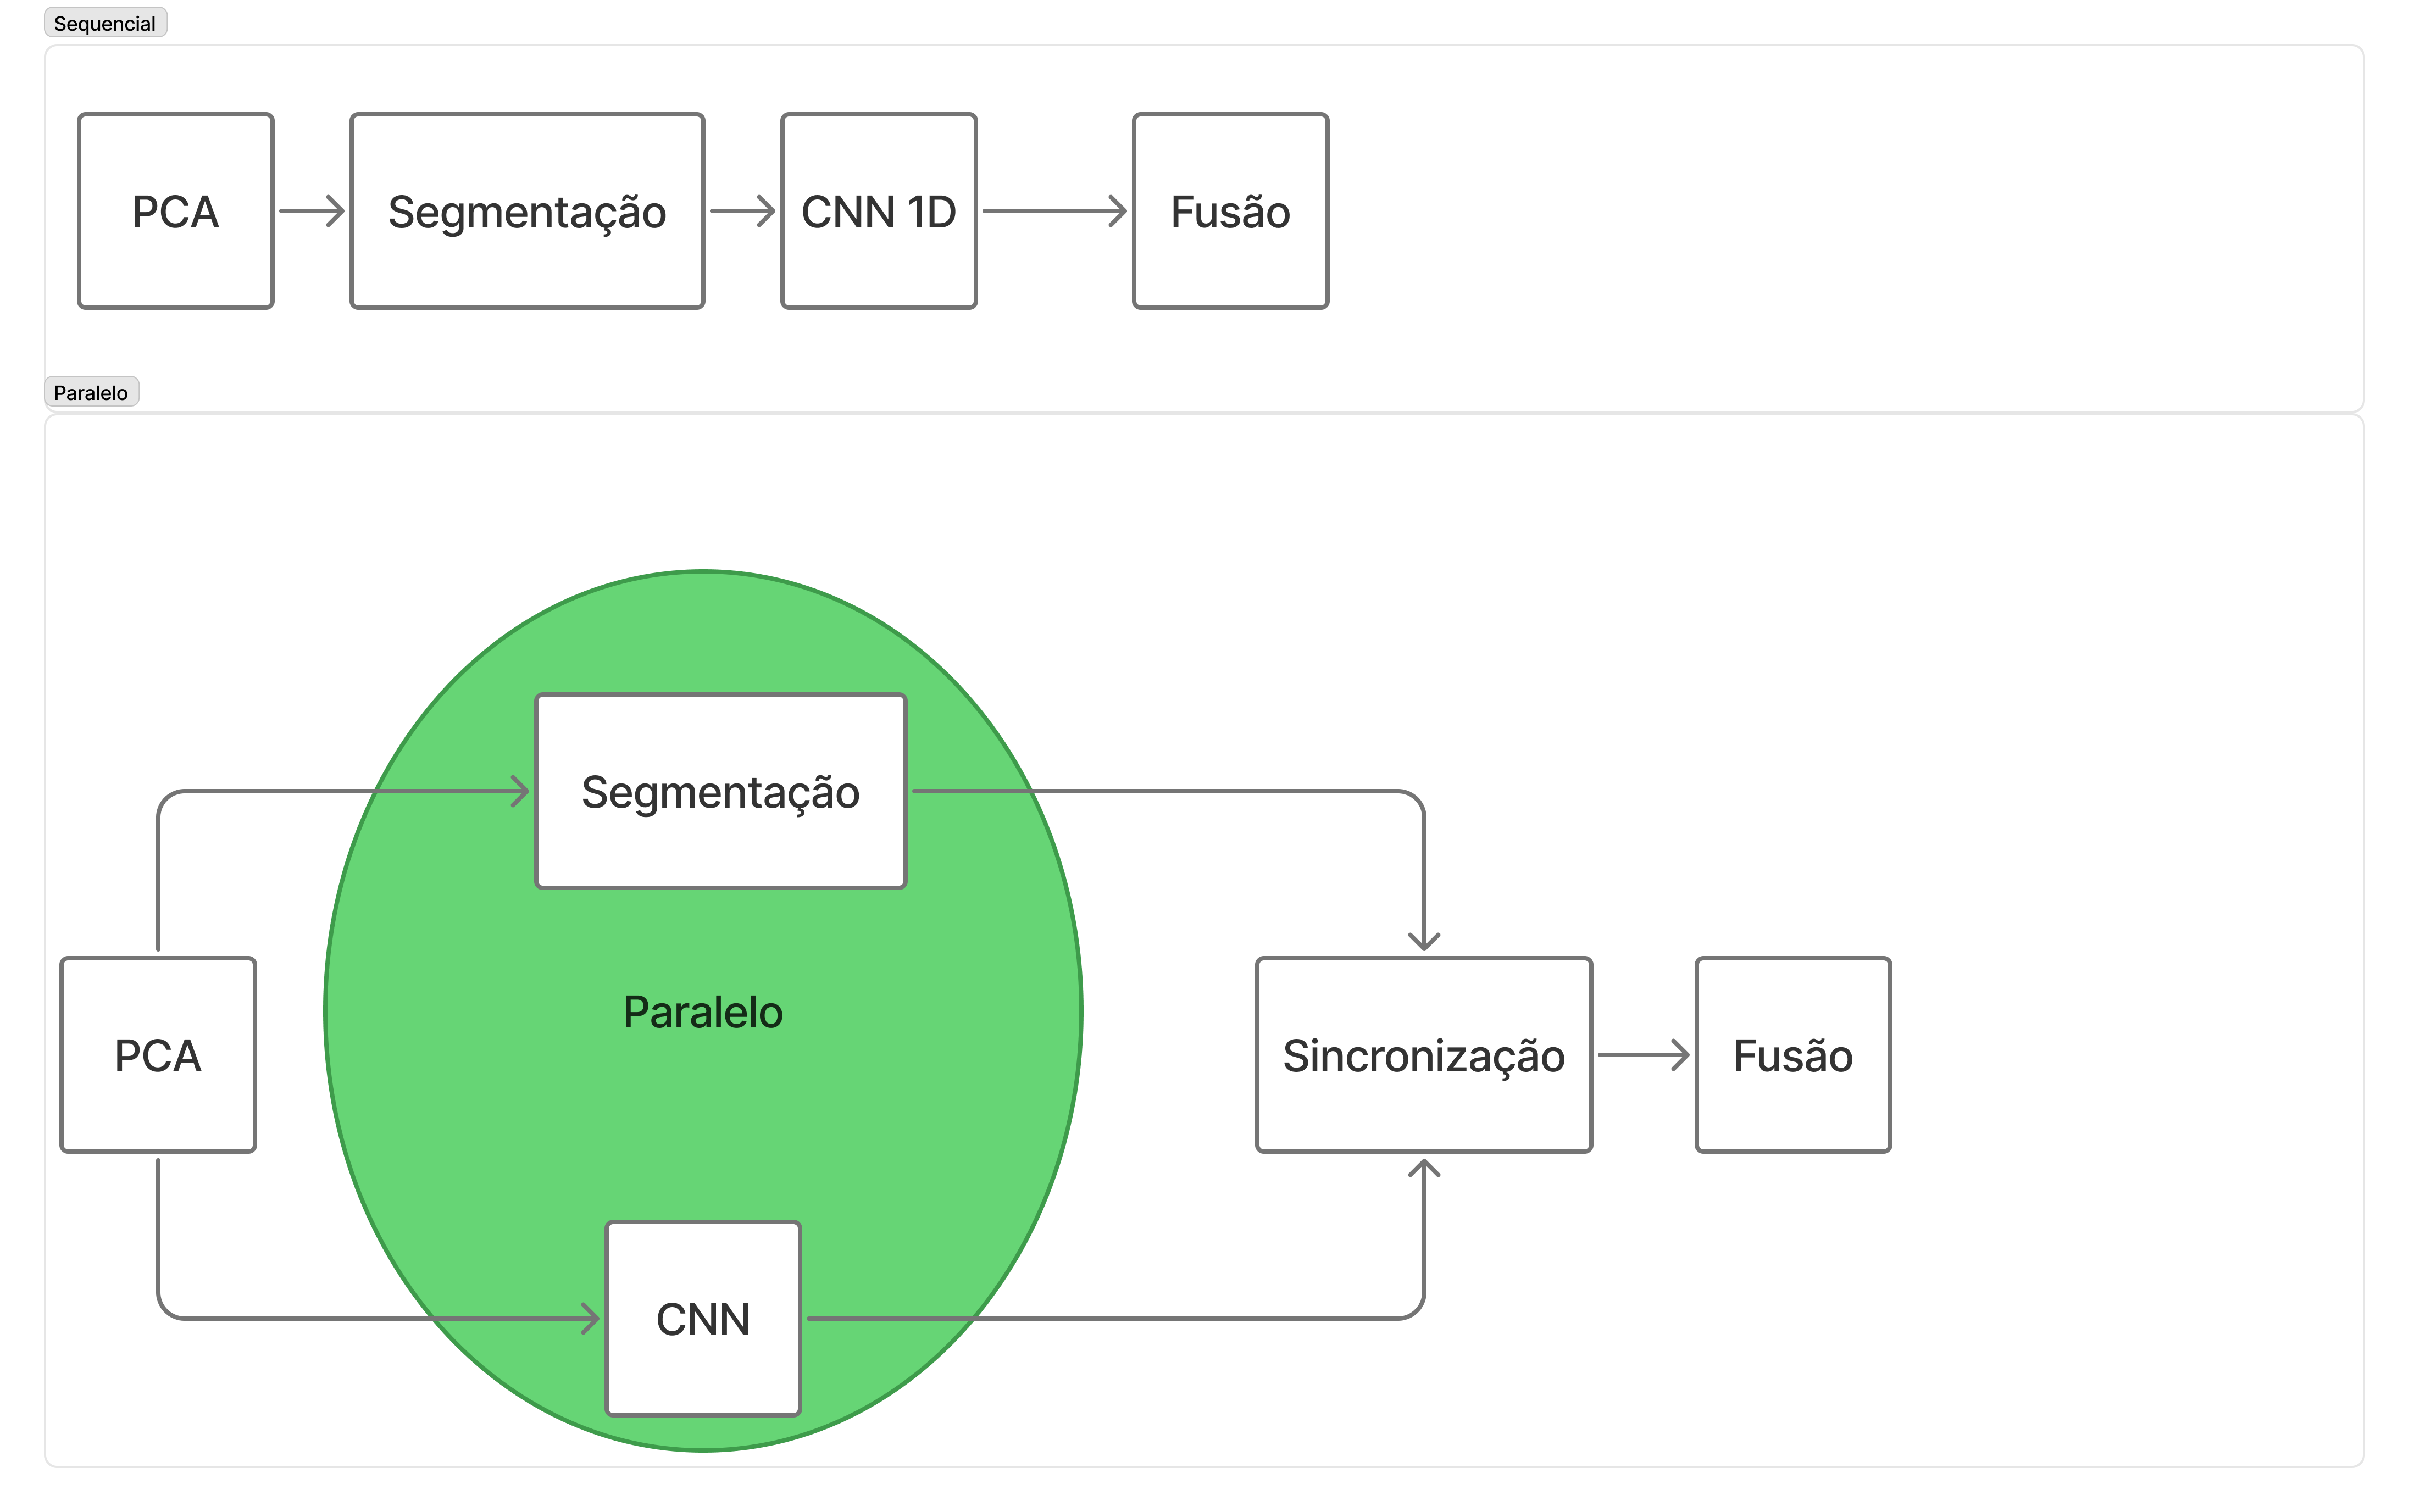
\includegraphics[width=0.7\textwidth]{assets/projeto/paralelizacao.png}\\
    \captionsetup{justification=raggedright}
    \caption*{Fonte: Elaborada pelo autor}
    \label{fig:paralelizacao}
\end{figure}

A Figura \ref{fig:paralelizacao} ilustra a diferença entre os dois fluxos de execução. No fluxo sequencial, após o PCA, a segmentação é executada primeiro, seguida pela CNN 1D, e então a fusão. No fluxo paralelo proposto, após o PCA, duas threads de execução são iniciadas concorrentemente: uma executa a segmentação espacial enquanto a outra executa a CNN 1D. A sincronização ocorre apenas no ponto de fusão. O speedup esperado é determinado pelo maior tempo entre as duas operações paralelas, acrescido da sobrecarga de gerenciamento de threads.

\subsubsection{Otimização Automática de Hiperparâmetros}

Duas abordagens de otimização serão implementadas:

\textbf{Grid Search}: Busca exaustiva em um espaço discreto de hiperparâmetros. Para cada combinação possível de parâmetros, um modelo é treinado e avaliado. Apesar de custoso computacionalmente, garante exploração completa do espaço de busca definido \cite{liashchynskyi2019gridsearchrandomsearch}.

\textbf{Otimização Bayesiana}: Abordagem mais eficiente que modela a função objetivo (acurácia de validação) como um processo Gaussiano e utiliza uma função de aquisição para decidir quais configurações testar a seguir, balanceando exploração e explotação \cite{WU201926}.

Os hiperparâmetros a serem otimizados incluem:

\textbf{Para a CNN 1D}: taxa de aprendizado, batch size, número de épocas, taxa de dropout, número de filtros por camada, tamanho dos kernels, otimizador (Adam, SGD, RMSprop).

\textbf{Para a Segmentação}: número de superpixels, número de iterações, parâmetros específicos de cada algoritmo.

\textbf{Para o PCA}: número de componentes principais.

\begin{figure}[H]
    \centering
    \captionsetup{justification=centering}
    \caption{Fluxo da otimização de hiperparâmetros}
    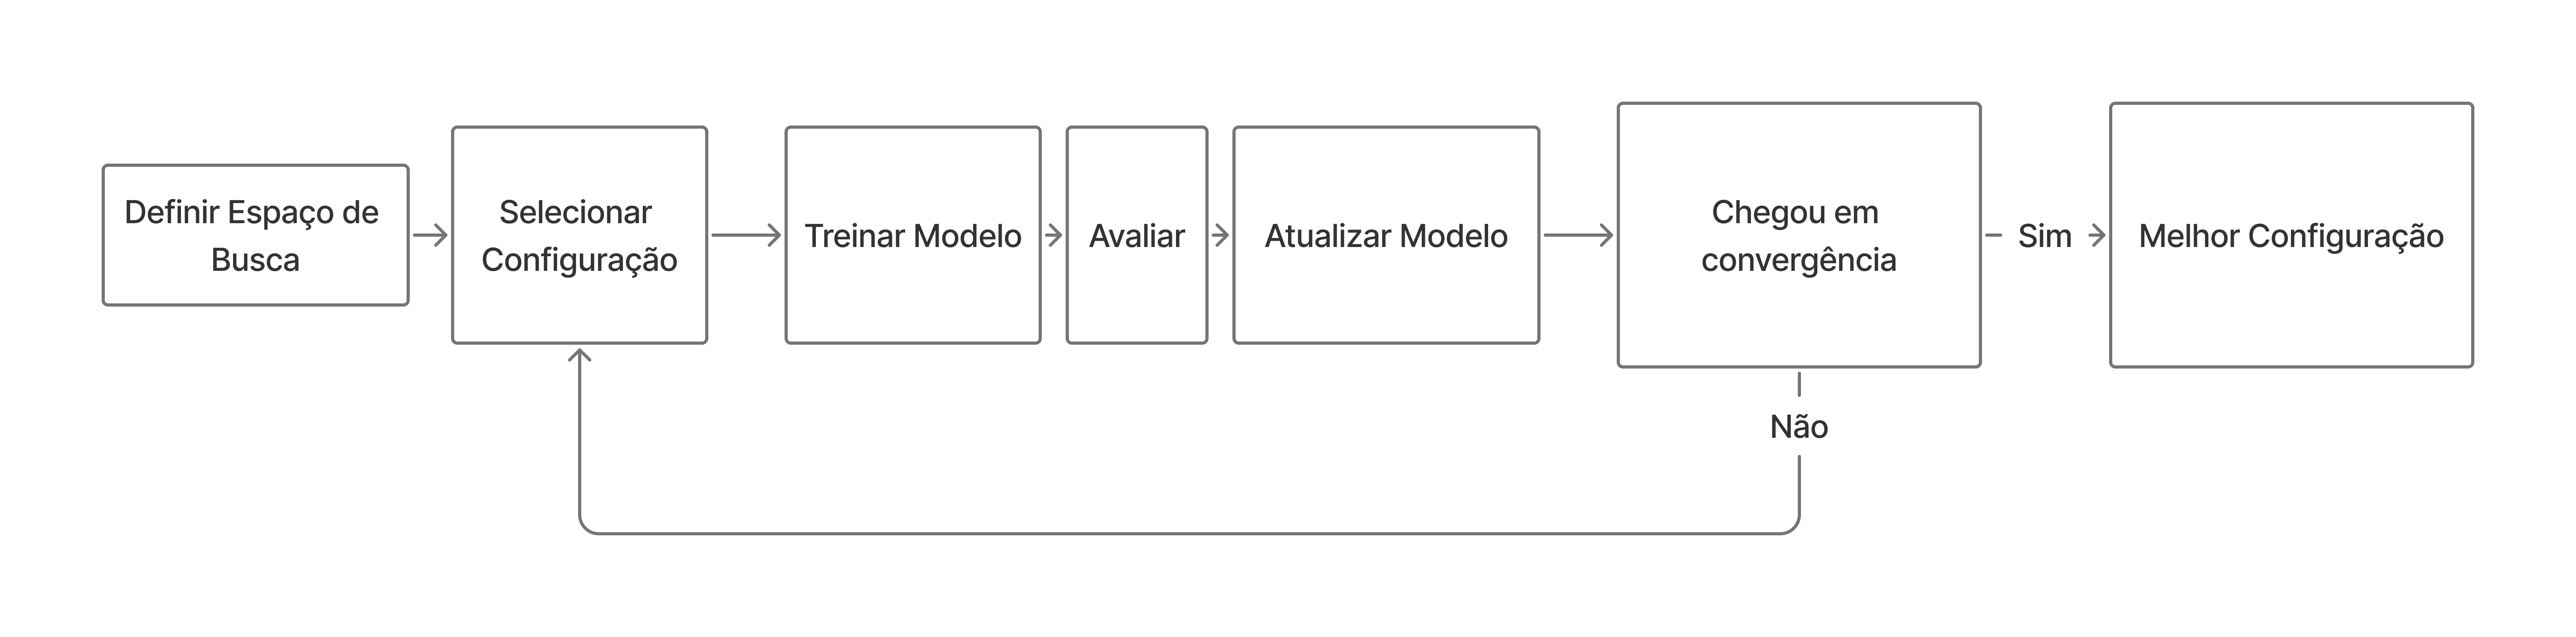
\includegraphics[width=0.7\textwidth]{assets/projeto/fluxoHPO.png}\\
    \captionsetup{justification=raggedright}
    \caption*{Fonte: Elaborada pelo autor}
    \label{fig:fluxoHPO}
\end{figure}

\section{Plano de Verificação}
\label{sec:planoVerificacao}

O plano de verificação estabelece um protocolo para validar o cumprimento dos requisitos estabelecidos e avaliar a eficácia das técnicas implementadas. A validação será conduzida através de uma campanha experimental, seguida de análise dos resultados obtidos. 

\subsection{Campanha Experimental}
\label{subsec:campanhaExperimental}

Será feito experimento para comparabilidade dos resultados e permitir análise incremental dos ganhos obtidos em cada etapa de otimização. A estratégia experimental tange uma abordagem progressiva, onde cada experimento constrói sobre os resultados do anterior, permitindo isolar e quantificar o impacto individual de cada técnica implementada.

Para cada dataset (Indian Pines, Salinas Valley e University of Pavia), serão realizados cinco experimentos principais, conforme detalhado na \autoref{tab:descricaoExperimentos}. Esta sequência experimental permite estabelecer uma linha de base e avaliar o impacto de cada componente do sistema proposto.


\begin{quadro}[H]
    \centering
    \caption{Descrição detalhada dos experimentos}
    \begin{tabular}{|p{0.18\textwidth}|p{0.72\textwidth}|}
        \hline
        \rowcolor[HTML]{C0C0C0}
        \textbf{Experimento} & \textbf{Descrição} \\
        \hline
        
        \textbf{Exp. 1 - Baseline} & Reprodução da arquitetura original sem otimizações (CNN 1D + SEEDS com parâmetros fixos, processamento sequencial) para estabelecer linha de base \\
        \hline
        
        \textbf{Exp. 2 - Otimização de Segmentação} & Teste dos três algoritmos de segmentação (SEEDS, LSC, Watershed) com otimização automática de seus parâmetros, mantendo CNN fixa \\
        \hline
        
        \textbf{Exp. 3 - Otimização de CNN} & Otimização dos hiperparâmetros da CNN 1D mantendo segmentação fixa \\
        \hline
        
        \textbf{Exp. 4 - Otimização Conjunta} & Otimização simultânea dos hiperparâmetros de segmentação e CNN \\
        \hline
        
        \textbf{Exp. 5 - Paralelização} & Aplicação da estratégia de paralelização sobre a melhor configuração identificada \\
        \hline
    \end{tabular}
    \label{tab:descricaoExperimentos}
\end{quadro}

Para cada experimento, serão realizadas 5 execuções independentes com diferentes seeds aleatórias para avaliar a variabilidade dos resultados. As métricas coletadas serão:

\begin{itemize}
    \item Acurácia Global (OA), Acurácia Média (AA), coeficiente Kappa
    \item Tempo de pré-processamento (PCA + Segmentação)
    \item Tempo de treinamento da CNN
    \item Tempo de inferência (total e por pixel)
    \item Uso de memória (pico durante treinamento e inferência)
    \item Número de parâmetros do modelo
    \item Speedup obtido com paralelização
\end{itemize}

Os resultados serão organizados conforme \autoref{tab:planejamentoExperimentos}.

\begin{quadro}[H]
    \centering
    \caption{Planejamento de experimentos}
    \begin{tabular}{|p{0.20\textwidth}|p{0.12\textwidth}|p{0.15\textwidth}|p{0.12\textwidth}|p{0.12\textwidth}|p{0.12\textwidth}|}
        \hline
        \rowcolor[HTML]{C0C0C0}
        \textbf{Experimento} & \textbf{Dataset} & \textbf{Segmentação} & \textbf{HPO CNN} & \textbf{HPO Seg.} & \textbf{Paralelo} \\
        \hline
        
        Exp1 - Baseline & IP, SV, UP & SEEDS & - & - & - \\
        \hline
        
        Exp2 - Otim. Seg. & IP, SV, UP & SEEDS/LSC/WS & - & X & - \\
        \hline
        
        Exp3 - Otim. CNN & IP, SV, UP & SEEDS & X & - & - \\
        \hline
        
        Exp4 - Otim. Conjunta & IP, SV, UP & Melhor & X & X & - \\
        \hline
        
        Exp5 - Paralelização & IP, SV, UP & Melhor & X & X & X \\
        \hline
    \end{tabular}
    \label{tab:planejamentoExperimentos}
\end{quadro}

\subsection{Análise Estatística dos Resultados}

Para cada conjunto de experimentos, será realizada análise estatística apropriada. A comparação entre diferentes configurações utilizará testes de significância estatística.

\subsection{Validação dos Requisitos}

A validação dos requisitos funcionais e não funcionais estabelecidos na \autoref{sec:req} será conduzida através de procedimentos específicos para cada requisito, conforme detalhado nas \autoref{tab:planoVerificacaoRF} e \autoref{tab:planoVerificacaoRNF}. Para cada requisito, são especificados os aspectos a serem validados, os métodos de validação a serem empregados e os critérios objetivos de sucesso.

\begin{quadro}[H]
    \centering
    \caption{Plano de verificação dos requisitos funcionais}
    \begin{tabular}{|p{0.08\textwidth}|p{0.25\textwidth}|p{0.35\textwidth}|p{0.22\textwidth}|}
        \hline
        \rowcolor[HTML]{C0C0C0}
        \textbf{Req.} & \textbf{Aspecto a Validar} & \textbf{Método de Validação} & \textbf{Critério de Sucesso} \\
        \hline
        
        \textbf{RF01} & Implementação correta da CNN 1D para extração de características espectrais & Testes verificando dimensões dos tensores em cada camada & Dimensões corretas em todas as camadas, gradientes computados adequadamente, resultados reprodutíveis \\
        \hline
        
        \textbf{RF02} & Implementação correta dos algoritmos de segmentação espacial & Testes verificando geração de mapas de superpixels & Mapas de segmentação gerados corretamente para os três algoritmos \\
        \hline
        
        \textbf{RF03} & Sistema de fusão por concatenação funcionando & Verificação das dimensões das características fusionadas correspondendo à soma das dimensões espectrais e espaciais & Fusão executada corretamente e classificação com fusão superior à classificação puramente espectral \\
        \hline
        
        \textbf{RF04} & Sistema de otimização automática de hiperparâmetros & Comparação entre algoritmos, verificando convergência e qualidade das configurações encontradas & Algoritmos convergem para configurações competitivas e pertinentes \\
        \hline
        
        \textbf{RF05} & Produção de métricas de desempenho e custo computacional & Coleta e registro de todas as métricas especificadas & Todas as métricas coletadas e registradas para análise comparativa \\
        \hline
        
        \textbf{RF06} & Eficácia da paralelização do processamento & Medição do tempo de execução com e sem paralelização, cálculo do speedup obtido & Redução mensurável no tempo de processamento \\
        \hline
    \end{tabular}
    \label{tab:planoVerificacaoRF}
\end{quadro}

\begin{quadro}[H]
    \centering
    \caption{Plano de verificação dos requisitos não funcionais}
    \begin{tabular}{|p{0.08\textwidth}|p{0.25\textwidth}|p{0.35\textwidth}|p{0.22\textwidth}|}
        \hline
        \rowcolor[HTML]{C0C0C0}
        \textbf{Req.} & \textbf{Aspecto a Validar} & \textbf{Método de Validação} & \textbf{Critério de Sucesso} \\
        \hline
        
        \textbf{RNF01} & Conformidade da arquitetura CNN 1D com o modelo base & Comparação estrutural com a arquitetura proposta por \cite{Souza2023} e \cite{Viel10064297} & Arquitetura implementada segue o modelo base especificado \\
        \hline
        
        \textbf{RNF02} & Desenvolvimento em Python & Verificação de que todos os módulos foram desenvolvidos em Python & Maior parte do código implementado em Python \\
        \hline
        
        \textbf{RNF03} & Utilização de plataforma adequada para treinamento & Confirmação de uso de Google Colab ou ambiente HPC com GPU & Experimentos executados em ambiente com aceleração por GPU \\
        \hline
        
        \textbf{RNF04} & Fusão por concatenação implementada corretamente & Verificação de que características espectrais e espaciais são concatenadas & Fusão realizada por concatenação de vetores \\
        \hline
        
        \textbf{RNF05} & Melhoria das métricas com otimização automática & Comparação das métricas OA, AA e Kappa entre configurações otimizadas automaticamente e ajuste manual & Métricas de acurácia superiores com otimização automática \\
        \hline
        
        \textbf{RNF06} & Reprodutibilidade dos resultados & Execução de múltiplas rodadas com mesmas configurações e análise de variabilidade & Desvio padrão das métricas inferior a 2\% entre execuções independentes \\
        \hline
        
        \textbf{RNF07} & Ganho de desempenho com paralelização & Medição quantitativa do speedup obtido & Redução mensurável no tempo em relação à implementação sequencial \\
        \hline
    \end{tabular}
    \label{tab:planoVerificacaoRNF}
\end{quadro}

É fundamental verificar se o sistema alcança desempenho satisfatório nos datasets de referência estabelecidos pela literatura. A \autoref{tab:validacaoDatasets} estabelece os valores baseline de acurácia que o sistema otimizado deve atingir ou superar para serem bem-sucedido. Estes valores foram extraídos dos resultados reportados em \cite{Souza2023} e trabalhos relacionados da literatura recente.


\begin{quadro}[H]
    \centering
    \caption{Validação de desempenho nos datasets de referência}
    \resizebox{\textwidth}{!}{%
    \begin{tabular}{|p{0.18\textwidth}|p{0.28\textwidth}|p{0.28\textwidth}|p{0.20\textwidth}|}
        \hline
        \rowcolor[HTML]{C0C0C0}
        \textbf{Dataset} & \textbf{Aspecto a Validar} & \textbf{Método de Validação} & \textbf{Baseline} \\
        \hline
        
        \textbf{Indian Pines} & 
        Métricas OA, AA e Kappa comparáveis ou superiores aos baselines & 
        Comparação com resultados de \cite{Souza2023} e trabalhos relacionados & 
        $OA \geq 95\%$, $AA \geq 93\%$, $Kappa \geq 0.94$ \\
        \hline
        
        \textbf{Salinas Valley} & 
        Métricas OA, AA e Kappa comparáveis ou superiores aos baselines & 
        Comparação com resultados de \cite{Souza2023} e trabalhos relacionados & 
        $OA \geq 97\%$, $AA \geq 96\%$, $Kappa \geq 0.96$ \\
        \hline
        
        \textbf{University of Pavia} & 
        Métricas OA, AA e Kappa comparáveis ou superiores aos baselines & 
        Comparação com resultados de \cite{Souza2023} e trabalhos relacionados & 
        $OA \geq 98\%$, $AA \geq 97\%$, $Kappa \geq 0.97$ \\
        \hline
    \end{tabular}%
    }
    \label{tab:validacaoDatasets}
\end{quadro}

\section{Análise de Riscos} 
\label{sec:analiseRiscos}

A análise de riscos identifica potenciais problemas que podem impactar o desenvolvimento e execução do projeto, estabelecendo estratégias de mitigação para cada cenário. O trabalho constrói sobre fundações técnicas estabelecidas na literatura, apresentando risco geral moderado.

O \autoref{tab:riscos} apresenta os principais riscos identificados, classificados quanto à probabilidade de ocorrência e impacto potencial no projeto.

\begin{quadro}[H]
    \centering
    \caption{Análise de riscos}
    \begin{tabular}{|p{0.22\textwidth}|p{0.12\textwidth}|p{0.10\textwidth}|p{0.46\textwidth}|}
        \hline
        \rowcolor[HTML]{C0C0C0}
        \textbf{Risco} & \textbf{Probab.} & \textbf{Impacto} & \textbf{Mitigação} \\
        \hline

        Tempo de HPO excede cronograma & Média & Alto & Reduzir espaço de busca e limitar número máximo de avaliações \\
        \hline

        Recursos computacionais insuficientes & Baixa & Médio & Utilizar Google Colab Pro, reduzir batch size, otimizar código \\
        \hline

        Dificuldade de reproduzir baseline & Média & Médio & Contatar autores originais, ajustar hiperparâmetros cuidadosamente \\
        \hline

        Variabilidade alta nos resultados & Média & Médio & Aumentar número de execuções, fixar seeds, analisar causas \\
        \hline
    \end{tabular}
    \label{tab:riscos}
\end{quadro}

\section{Cronograma}

O cronograma apresentado na \autoref{tab:cronograma} distribui as atividades do TCC ao longo do primeiro semestre de 2026. A escrita da monografia é uma atividade contínua. As implementações seguem ordem de dependências. Os experimentos são concentrados na segunda metade do período.

\begin{quadro}[H]
    \centering
    \caption{Cronograma de atividades do TCC}
    \begin{tabular}{|p{0.40\textwidth}|c|c|c|c|c|c|}
    \hline
    \rowcolor[HTML]{C0C0C0}
    \textbf{Atividade} & \textbf{Jan} & \textbf{Fev} & \textbf{Mar} & \textbf{Abr} & \textbf{Mai} & \textbf{Jun} \\
    \hline
    Escrita da Monografia & X & X & X & X & X & - \\
    \hline
    Implementação (CNN 1D, Segmentação, Fusão) & X & X & - & - & - & - \\
    \hline
    Implementação do Sistema de HPO & - & X & X & - & - & - \\
    \hline
    Implementação da Paralelização & - & - & X & - & - & - \\
    \hline
    Experimentos e Coleta de Métricas & - & - & X & X & X & - \\
    \hline
    Análise dos Resultados & - & - & - & - & X & X \\
    \hline
    Revisão Textual e Apresentação & - & - & - & X & X & X \\
    \hline
    \end{tabular}
    \label{tab:cronograma}
\end{quadro}